\begin{description}
    \item[Vereinigung] $A \cup B = \lbrace x | x \in A \vee x \in B \rbrace$ \\
    \begin{tabular}{l|l|l}
        \adjustbox{valign = t}{
            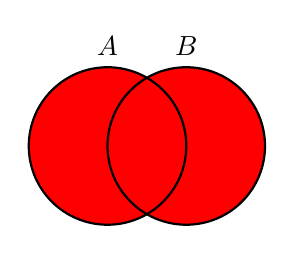
\begin{tikzpicture}[thick, set/.style = {circle, minimum size = 2cm, fill=red}]
                \node [set, label={90:$A$}] (A) at (-0.5,0) {};
                \node [set, label={90:$B$}] (B) at (0.5,0) {};
                \draw (-0.5,0) circle(1);
                \draw (0.5,0) circle(1);
            \end{tikzpicture}
        }                                                               &
        \adjustbox{valign = t}{
            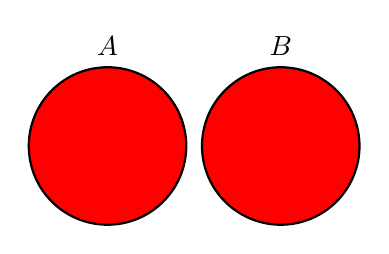
\begin{tikzpicture}[thick, set/.style = {circle, minimum size = 2cm, draw = black, fill=red}]
                \node [set, label={90:$A$}] (A) at (-1.1,0) {};
                \node [set, label={90:$B$}] (B) at (1.1,0) {};
            \end{tikzpicture}} &
        $\begin{array}{r c l}
             |A \cup B| & = & |A| + |B \setminus A| \\
             & = & |B| + |A \setminus B|
        \end{array}$
    \end{tabular}
    \item[Durchschnitt] $A \cap B \coloneqq \lbrace x | x \in A \wedge x \in B \rbrace$ \\
    \begin{tabular}{l|l|l}
        \adjustbox{valign = t}{
            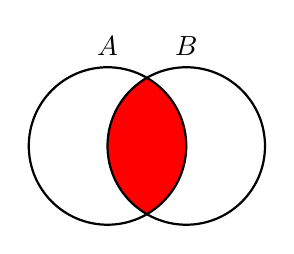
\begin{tikzpicture}[thick, set/.style = {circle, minimum size = 2cm, draw = black}]
                \begin{scope}
                    \clip (-0.5,0) circle(1);
                    \fill[red] (0.5, 0) circle (1);
                \end{scope}
                \node [set, label={90:$A$}] (A) at (-0.5,0) {};
                \node [set, label={90:$B$}] (B) at (0.5,0) {};
            \end{tikzpicture}
        } &
        \adjustbox{valign = t}{
            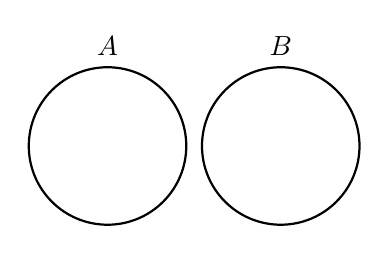
\begin{tikzpicture}[thick, set/.style = {circle, minimum size = 2cm, draw = black}]
                \node [set, label={90:$A$}] (A) at (-1.1,0) {};
                \node [set, label={90:$B$}] (B) at (1.1,0) {};
            \end{tikzpicture}
        } &
        $\begin{array}{r c l}
             |A \cap B| & = & |A| - |A \setminus B| \\
             & = & |B| - |B \setminus A|
        \end{array}$
    \end{tabular}
    \item[Mengendifferenz] $A \setminus B = \lbrace x | x \in A \wedge x \not \in B \rbrace$ \\
    \begin{tabular}{l|l|l}
        \adjustbox{valign = t}{
            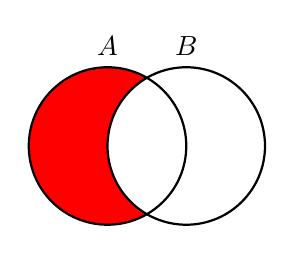
\begin{tikzpicture}[thick, set/.style = {circle, minimum size = 2cm, draw = black}]
                \begin{scope} [even odd rule]
                    \clip (-0.5,0) circle(1) (0.5,0) circle(1);1
                    \fill [red] (-0.5,0) circle (1);
                \end{scope}
                \node [set, label={90:$A$}] (A) at (-0.5,0) {};
                \node [set, label={90:$B$}] (B) at (0.5,0) {};
            \end{tikzpicture}
        } &
        \adjustbox{valign = t}{
            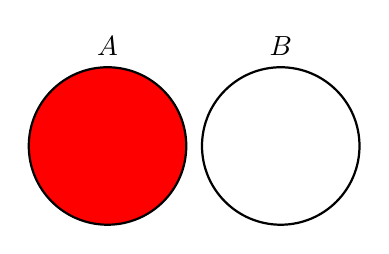
\begin{tikzpicture}[baseline=(current bounding box.north), thick, set/.style = {circle, minimum size = 2cm, draw = black}]
            \node [set, fill = red, label={90:$A$}] (A) at (-1.1,0) {};
            \node [set, label={90:$B$}] (B) at (1.1,0) {};
            \end{tikzpicture}
        } &
    \end{tabular}
    \item[symmetrische Differenz] $A \Delta B = (A \setminus B) \cup (B \setminus A)$ \\
    \begin{tabular}{l|l|l}
        \adjustbox{valign = t}{
            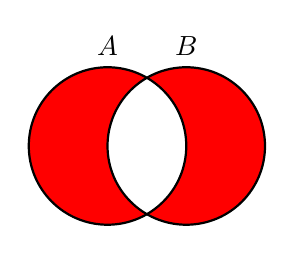
\begin{tikzpicture}[thick, set/.style = {circle, minimum size = 2cm, draw = black}]
                \fill [even odd rule, red] (-0.5,0) circle (1) (0.5,0) circle (1);
                \node [set, label={90:$A$}] (A) at (-0.5,0) {};
                \node [set, label={90:$B$}] (B) at (0.5,0) {};
            \end{tikzpicture}
        } &
        \adjustbox{valign = t}{
            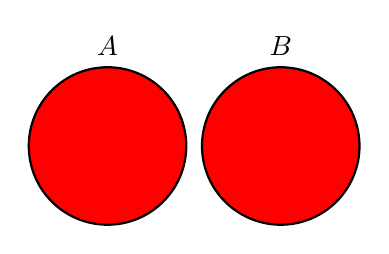
\begin{tikzpicture}[baseline=(current bounding box.north), thick, set/.style = {circle, minimum size = 2cm, draw = black, fill = red}]
            \node [set, label={90:$A$}] (A) at (-1.1,0) {};
            \node [set, label={90:$B$}] (B) at (1.1,0) {};
            \end{tikzpicture}
        } &
        $|A \Delta B| = |A \setminus B| + |B \setminus A|$
    \end{tabular}
    \item[Potenzmengen] $\mathcal{P}(A) \coloneqq \lbrace B|B \subseteq A \rbrace;\ |\mathcal{P}(A)| = 2^{|A|}$
    \item[ungeordnets Paar] $\lbrace a,b \rbrace = \lbrace c,d \rbrace \Rightarrow (a=c \wedge b=d) \vee (a=d \wedge b=c)$
    \item[geordnetes Paar] $\lbrace a,b \rbrace = \lbrace c,d \rbrace \Rightarrow a=c \wedge b=d$ (Das geht!)
    \item[Mengenprodukt] $A \times B = \lbrace (a,b)|a \in A \wedge b \in B \rbrace$ (nicht Kommutativ, (strenggenommen) nicht assoziativ)
    \begin{align*}
    (A \times B)
        \times C & \not = A \times (B \times C) \\
        ((a,b),c)             & \not = (a,(b,c))
    \end{align*}
    Gegeben sein
    \begin{gather*}
        A = \lbrace 1, 2 \rbrace\\
        B = \lbrace a, b, c \rbrace\\
    \end{gather*}
    dann ist:
    \[A \times B = \lbrace (1,a),(2,a)(1,b)(2,b),(1,c)(2,c) \rbrace\] \\
    $|A \times B| = |A| \cdot |B|$
\end{description}
